% Asset ID: AS1AlgebraicMethodsProofTikZ-001
% Source: Chapter 7b Algebraic Methods, Proof transcript
% Related lesson section: Worked Example 5; Common Mistakes and Exam Traps
% Purpose: Right-triangle setup for proving consecutive integer side lengths must be 3, 4, 5.

\documentclass[tikz,border=8pt]{standalone}
\usepackage{amsmath}
\usetikzlibrary{arrows.meta,positioning,calc}
\begin{document}
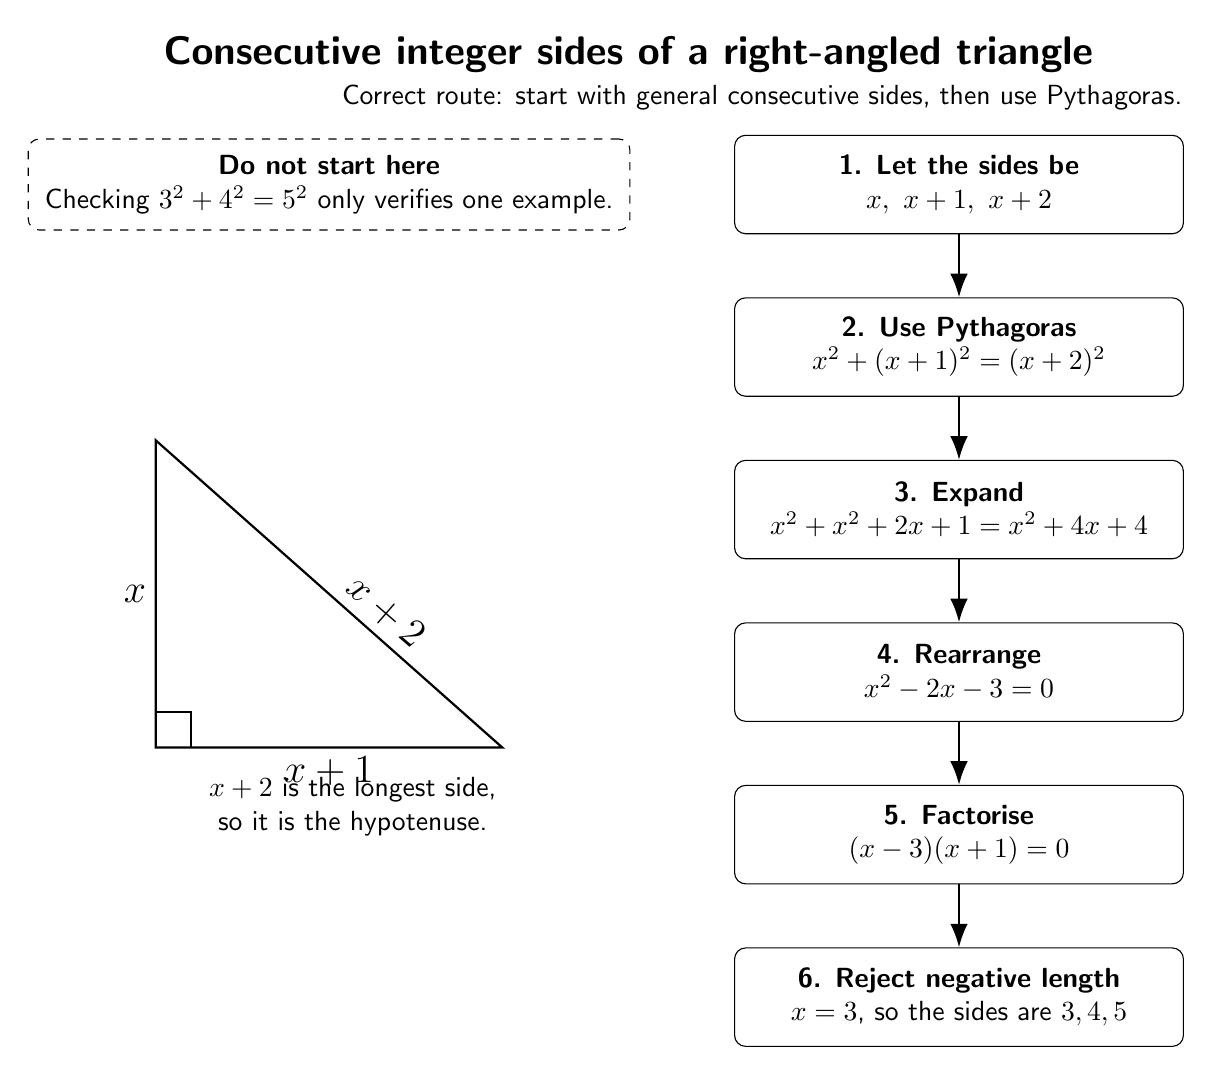
\begin{tikzpicture}[font=\sffamily,box/.style={draw,rounded corners,align=center,minimum width=5.7cm,minimum height=1.25cm,inner sep=6pt},warn/.style={draw,rounded corners,dashed,align=center,minimum width=6.2cm,minimum height=1.15cm,inner sep=6pt},arr/.style={-{Latex[length=3mm]}, thick}]
\node[align=left, font=\sffamily\bfseries\Large] at (0,7.2){Consecutive integer sides of a right-angled triangle};
\node[align=left] at (1.7,6.65){Correct route: start with general consecutive sides, then use Pythagoras.};
\node[warn] (bad) at (-3.8,5.55){\textbf{Do not start here}\\Checking \(3^2+4^2=5^2\) only verifies one example.};
\coordinate (A) at (-6,-1.6);\coordinate (B) at (-6,2.3);\coordinate (C) at (-1.6,-1.6);
\draw[thick] (A) -- (B) -- (C) -- cycle;\draw[thick] ($(A)+(0,0.45)$) -- ++(0.45,0) -- ++(0,-0.45);
\node[left] at ($(A)!0.5!(B)$) {\Large \(x\)};\node[below] at ($(A)!0.5!(C)$) {\Large \(x+1\)};\node[above right, rotate=-41] at ($(B)!0.5!(C)$) {\Large \(x+2\)};
\node[align=center] at (-3.5,-2.35){\(x+2\) is the longest side,\\so it is the hypotenuse.};
\node[box] (s1) at (4.2,5.55){\textbf{1. Let the sides be}\\\(x,\ x+1,\ x+2\)};
\node[box, below=0.8cm of s1] (s2){\textbf{2. Use Pythagoras}\\\(x^2+(x+1)^2=(x+2)^2\)};
\node[box, below=0.8cm of s2] (s3){\textbf{3. Expand}\\\(x^2+x^2+2x+1=x^2+4x+4\)};
\node[box, below=0.8cm of s3] (s4){\textbf{4. Rearrange}\\\(x^2-2x-3=0\)};
\node[box, below=0.8cm of s4] (s5){\textbf{5. Factorise}\\\((x-3)(x+1)=0\)};
\node[box, below=0.8cm of s5] (s6){\textbf{6. Reject negative length}\\\(x=3\), so the sides are \(3,4,5\)};
\draw[arr] (s1) -- (s2);\draw[arr] (s2) -- (s3);\draw[arr] (s3) -- (s4);\draw[arr] (s4) -- (s5);\draw[arr] (s5) -- (s6);
\end{tikzpicture}
\end{document}
